%%%%%%%%%%%%%%%%%%%%%%%%%%%%%%%%%%%%%%%%%
% a0poster Portrait Poster
% LaTeX Template
% Version 1.0 (22/06/13)
%
% The a0poster class was created by:
% Gerlinde Kettl and Matthias Weiser (tex@kettl.de)
% 
% This template has been downloaded from:
% http://www.LaTeXTemplates.com
%
% License:
% CC BY-NC-SA 3.0 (http://creativecommons.org/licenses/by-nc-sa/3.0/)
%
%%%%%%%%%%%%%%%%%%%%%%%%%%%%%%%%%%%%%%%%%

%----------------------------------------------------------------------------------------
%	PACKAGES AND OTHER DOCUMENT CONFIGURATIONS
%----------------------------------------------------------------------------------------

\documentclass[a0,portrait]{a0poster}

\usepackage{ wasysym } % astrosun symbol.
\usepackage{multicol} % This is so we can have multiple columns of text side-by-side
\columnsep=100pt % This is the amount of white space between the columns in the poster
\columnseprule=3pt % This is the thickness of the black line between the columns in the poster

\usepackage[svgnames]{xcolor} % Specify colors by their 'svgnames', for a full list of all colors available see here: http://www.latextemplates.com/svgnames-colors

%\usepackage{times} % Use the times font
\usepackage{palatino} % Uncomment to use the Palatino font

\usepackage{graphicx} % Required for including images
\graphicspath{{figures/}} % Location of the graphics files
%\usepackage{booktabs} % Top and bottom rules for table
\usepackage[font=small,labelfont=bf]{caption} % Required for specifying captions to tables and figures
%\usepackage{amsfonts, amsmath, amsthm, amssymb} % For math fonts, symbols and environments
%\usepackage{wrapfig} % Allows wrapping text around tables and figures

%\usepackage{realboxes}

\renewcommand{\emph}[1]{\textbf{\color{blue}#1}}
%\renewcommand{\section}[2]{\Colorbox{lightgray}{\noindent {\Large \textbf{#2}} \hfill}}

\usepackage{lipsum}

\begin{document}

%----------------------------------------------------------------------------------------
%	POSTER HEADER 
%----------------------------------------------------------------------------------------

% The header is divided into two boxes:
% The first is 75% wide and houses the title, subtitle, names, university/organization and contact information
% The second is 25% wide and houses a logo for your university/organization or a photo of you
% The widths of these boxes can be easily edited to accommodate your content as you see fit

\begin{minipage}[b]{0.75\linewidth}
  \Huge \textbf{Detectability study of EM/GW events with INTEGRAL.}\\[1cm] % Title
  \large \textbf{P.~Bacon$^{1}$ V.~Savchenko$^{1}$  E.~Chassande-Mottin$^{1}$}\\[1cm] % Author(s)
  \normalsize 1. APC, Univ Paris Diderot, CNRS/IN2P3, CEA/Irfu, Obs. de Paris, Sorbonne Paris Cit\'e, France\\
  \large \texttt{philippe.bacon@apc.in2p3.fr}\\
\end{minipage}
%
\begin{minipage}[b]{0.25\linewidth}
	
\includegraphics[width=20cm]{logo.png}
\end{minipage}

\vspace{1cm} % A bit of extra whitespace between the header and poster content

%----------------------------------------------------------------------------------------

\begin{multicols}{2} % This is how many columns your poster will be broken into, a portrait poster is generally split into 2 columns


 \begin{abstract}
%\lipsum[20]
On September 2015, the two LIGO interferometers realized the first direct detection of gravitational waves (GW) and opened a new era in astronomy history. A next step would be to detect some electromagnetic (EM) counterparts associated to GW events. Among them short gamma-ray bursts (SGRBs) produced by the coalescence of binary neutron stars are surely the most powerful sources detectable by high energy detectors. We thus address the question of the joint detectability of GW events by Advanced Virgo and Advanced LIGO interferometers, and EM events with the INTEGRAL satellite : what should be the statistical significance of the GW and the EM events to claim a joint detection ? \textcolor{blue}{BOTTOM LINE RESULTS : We show that...}
 \end{abstract}

\section*{Monte-Carlo simulation of GW events.}

%\lipsum
% SNR threshold HL = 6 : RHO_thres_NETWORK = sqrt(rho_H**2 + rho_L**2) = 6

\indent We used a catalogue of Milky Way-like galaxies in which populations of $Z_{\astrosun}$ metallicity binary neutron stars (BNS) systems have been simulated thanks to the Synthetic Universe database \cite{syntheticUniverse}. To do this we injected artificial GW signals corresponding to the coalescence of the two compact objects into O2b anticipated detector noise. On one hand, the signal only takes the inspiral phase into account via the use of non-spinning waveform 'TaylorF4ThreePN'. On the other hand, we took the O2b period to last for 3 months with a duty cycle of $50 \, \%$. Finally, we try to recover these fake GW signals using matched-filtering techniques thanks to the BAYESTAR pipeline. \\
\indent This detectability study echoes the one of Patricelli et al. \cite{2016arXiv160606124P} who used the \textsc{FERMI} instrument to monitor gamma-ray events. As we want to reproduce an analogue study with \textsc{INTEGRAL} it justifies why our simulation settings are aligned on their work. This will allow further comparisons. As a sanity check we found the SNR, inclination and sky distribution of the events to be qualitatively consistent with both Patricelli et al. and Dominik et al. \textcolor{blue}{Add ref ?}. \\
\textcolor{blue}{What to present ? HL ? HLV ? both ?} \\
\indent As a transition towards the details of the EM emission we estimated the total GW emitted energy $E_{\mathrm{EM}}$ of the simulated BNS systems thanks to Bernuzzi et al. \cite{2016PhRvD..94b4023B}, ie.  $E_{GW} \sim 1.5 \% \, M c^{2}$ where M is the total mass of the binary.

\section*{Assumptions on the EM emission.}

\indent First hard point is to properly articulate between EM and GW emission. For this we took a rather simple model. Indeed, is has been considered it exist a proportionality relation between $E_{GW}$ and $E_{\mathrm{EM}}$ \textcolor{blue}{ref ? justification ?}.
It has to be emphasized that every simulated GW event is associated to a gamma-ray event. As GRBs will then be monitored thanks to the SPI-ACS and IBIS instruments embarked on the \textsc{INTEGRAL} satellite mission, we thus have to convert the energy information into some constraints acting on the detectable energy flux by those instruments. The emitted EM flux is hence truncated to the \textsc{INTEGRAL} finite energy band $\left[ 75 \, , 2000 \right] \, \mathrm{keV}$. \\
\indent Observational evidences of GRBs EM emission generally show two kinds of emissions : a prompt emission in the gamma-ray or X-ray domain which corresponds to the collimated ejection of relativistic jet of matter, and an afterglow emission in the optic or radio domain produced after the ejecta has been slowed down by internally driven shocks between many layers. The former part is well modelled by the BAND emission spectrum with the following fixed parameters $\alpha_{\mathrm{BAND}} = - 0.5$, $\beta_{\mathrm{BAND}} = - 2.25$ and $E_{\mathrm{PEAK}} = 800 \, MeV$. The latter ... \textcolor{blue}{DESCRIBE AFTERGLOW}

\section*{Visibility.}

Estimate the visibility of the EM counterpart is equivalent to definite a follow-up strategy. It means to determine the fraction of the accessible sky region and how should we optimize both the exposure duration and the EM significance. \\
Considering a passive follow-up strategy, the actual orientations are due to the planned observation constraints (galactic plane, center, etc.). The fluences are computed assuming a fixed beaming angle of $10 \, \mathrm{deg}$ for a $1 \, s$-long emission. \textcolor{blue}{fig ?}. The SPI-ACS and IBIS/Veto instruments show a complementary in the covered sky region. \textcolor{blue}{fig ?}
%Should INTEGRAL follow its observation plan and re-point while asked by LIGO/Virgo triggers ?
%How the follow-up strategy will be determined depends on the sky region area.
%\textcolor{blue}{PUT PLOT RATE OF DETECTIONS IN MONTHS VS. SIGNIFICANCE}
%We are able to recover 25 \% of the events in a 6-months run with a 5 sigma significance if we assume INTEGRAL stay focus during 0.5 day on a given source.


\section*{Detectability.}

\section*{Results.}

%\lipsum[20]

\section*{Discussion.}

%\lipsum[20]

%\begin{center}\vspace{.5cm}
%    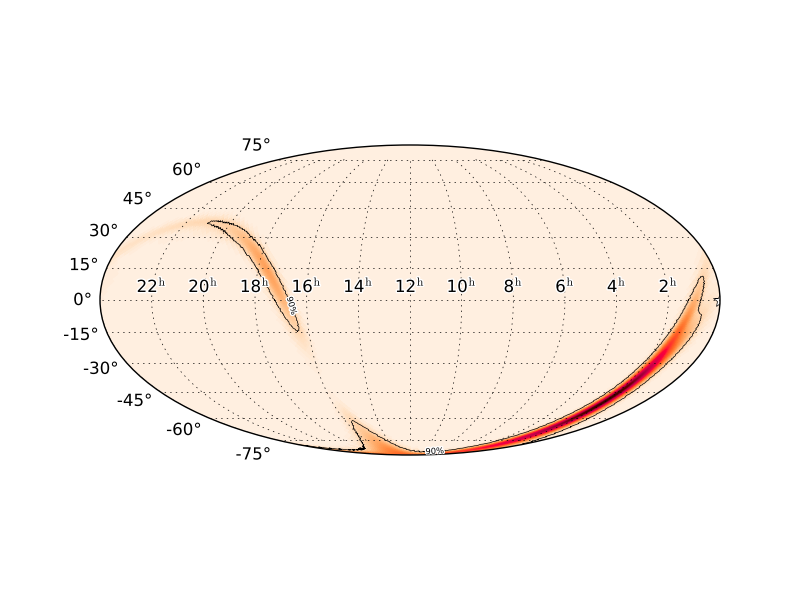
\includegraphics[height=20cm]{figures/test.png}
%    \captionof{figure}{test}
%\end{center}

\cite{*}

%----------------------------------------------------------------------------------------
%	ACKNOWLEDGEMENTS
%----------------------------------------------------------------------------------------

\vspace{10mm}
\noindent {\normalsize \textbf{Acknowledgements}}

{\footnotesize 
  We thank ASTERICS. Barbara Patricelli for sharing data, Philippe Laurent for discussions}

%----------------------------------------------------------------------------------------
%	REFERENCES
%----------------------------------------------------------------------------------------

%\nocite{*} % Print all references regardless of whether they were cited in the poster or not
\bibliographystyle{plain} % Plain referencing style
\bibliography{reference_phil} % Use the example bibliography file sample.bib

%----------------------------------------------------------------------------------------

\end{multicols}
\end{document}